\subsection{Ondas estacionárias de som: geração de harmônicos em
função do comprimento L}

Neste experimento, a frequência de excitação $f$ foi fixada em aproximadamente 2 KHz (mais precisamente 2,0004 KHz com precisão de 0,0001 KHz) e os harmônicos foram gerados com a variação do comprimento L da coluna de ar. Ao deslocar o pistão, observou-se que em certas posições $L_n$, as ondas de pressão atingiram intensidades máximas. Quando isso acontecia, registrava-se a posição do pistão. Após 5 leituras, construímos a seguinte tabela com os dados:

\begin{table}[H]
    \centering
    \begin{tabular}{ |c||c||c|}
        \hline
        \textbf{Índice harmônico \textit{n}} & \textbf{Comprimento Coluna de Ar \textit{$L_n$}(m)} & \textbf{$L_{n+1} - L_n$ (m)}\\
        \hline 
         1&	0,080&	----	\\
         
         2&	0,165&	0,085 \\
         
         3&	0,252&	0,087 \\
         
         4&	0,340&	0,088 \\
         
         5&	0,426&	0,086 \\
        \hline
    \end{tabular}
    \caption{Tabela registrando os valores do índice \textit{n} do harmônico, o comprimento da coluna de ar deslocado \textit{$L_n$} e \textit{$L_{n+1} - L_n$}.}
\end{table}

Com base na equação $n \cdot \frac{\lambda_n}{2}=L$, espera-se que os valores obtidos sejam aproximadamente iguais à metade do valor do comprimento de onda , pois, sabendo que o comprimento de onda  é constante, ao manipular a equação temos que:

\[ L_n = n \cdot \frac{\lambda_n}{2}\] 
\[L_{n+1} = (n+1) \cdot \frac{\lambda_n}{2}\]

\[L_{n+1} - L_n = (n+1) \cdot \frac{\lambda_n}{2} - n \cdot \frac{\lambda_n}{2}\] 
\[L_{n+1} - L_n = n \cdot \frac{\lambda_n}{2} - n \cdot \frac{\lambda_n}{2} + \frac{\lambda_n}{2}\] 
\[\therefore L_{n+1} - L_n = \frac{\lambda_n}{2}\] 

Feito essa análise, determinamos o valor do comprimento de onda $\lambda$ com sua respectiva incerteza para verificar se a condição acima é satisfeita. Por meio da fórmula $\lambda = \frac{2 \cdot L_n}{n}$  pudemos, então, calcular o valor de $\lambda_m \pm \Delta\lambda$. Os valores utilizados para esse cálculo estão expressos abaixo e na Tabela logo em seguida:

\[ \lambda_1 = 2 \cdot \frac{0,080}{1} \ \to \ \lambda _1 = 0,160 m  \]
\[ \lambda_2 = 2 \cdot \frac{0,165}{2} \ \to \ \lambda _2 = 0,165 m  \]
\[ \lambda_3 = 2 \cdot \frac{0,252}{3} \ \to \ \lambda _3 = 0,168 m  \]
\[ \lambda_4 = 2 \cdot \frac{0,340}{4} \ \to \ \lambda _4 = 0,170 m  \]
\[ \lambda_5 = 2 \cdot \frac{0,426}{5} \ \to \ \lambda _5 = 0,170 m  \]

\begin{table}[H]
    \centering
    \begin{tabular}{ |c||c| }
        \hline
        \textbf{Índice do harmônico \textit{n}} & \textbf{Comprimento de Onda \textit{$\lambda_n$}(m)}\\
        \hline 
         1&	0,160 \\
         
         2&	0,165 \\
         
         3&	0,168 \\
         
         4&	0,170 \\
         
         5&	0,170 \\
        \hline
    \end{tabular}
    \caption{Tabela registrando os valores do índice \textit{n} do harmônico com o comprimento de onda $\lambda_n$ correspondente.}
\end{table}

Portanto, a partir do cálculo da média dos comprimentos de onda, chegamos nos seguintes valores:

\[ \lambda = \frac{\sum \lambda_i}{5} = \frac{0,8334}{5} = 0,167 m\] 
\[ \Delta\lambda = \frac{\sum |\lambda_i - \lambda|}{5} = \frac{0,01632}{5} = 0,003 m\] 

\[ \therefore \lambda = (0,167 \pm 0,003)m\] 

Com base no valor encontrado para o comprimento de onda, podemos comprovar se $L_{n+1} - L_n$ corresponde à metade de $\lambda$:

\[ L_{n+1} - L_n = 0,085 m\]

\[ \frac{\lambda}{2} = \frac{0,167}{2} = 0,0835 m\]
\[ \frac{\Delta\lambda}{2} = \frac{0,003}{2} = 0,0015 m\]
\[ \frac{\lambda}{2} = (0,084 \pm 0,002) m\]

\[ \therefore L_{n+1} - L_n = \frac{\lambda}{2} \]

Dando prosseguimento ao experimento, também calculamos a velocidade de propagação do som no ar:

\[ v = (\lambda_m \pm \Delta\lambda) \cdot (f \pm \Delta f)\]
\[ v = (0,167 \pm 0,003) \cdot (2000,4 \pm \Delta 0,1)\]
\[ \therefore v = (334 \pm 6) m/s\]

Frente a velocidade calculada, pode-se concluir que esta é, dentro da sua margem de erro, não correspondente a velocidade de referência da propagação do som no ar (343m/s). Essa não correspondência pode ser atribuída a uma diferença mínima entre os valores gerada por erros sistemáticos ao longo do experimento, como leitura incorreta da régua ou pequenas dispersões de dados. Entretanto, para efeito experimental, por chegarmos a um valor muito próximo da referência, podemos afirmar que o resultado é satisfatório.\\

Para complementar, além dos cálculos realizados, também podemos encontrar a velocidade do som no ar para o experimento a partir de uma análise gráfica que relaciona o comprimento L em função do quociente $n/2L$. Semelhante ao experimento anterior, se aplicarmos o método dos mínimos quadrados, podemos encontrar o coeficiente angular que coincide exatamente com a velocidade da onda. Então, realizando esses dois processos, temos os gráficos abaixo:

\begin{figure}[H]
  \centering
  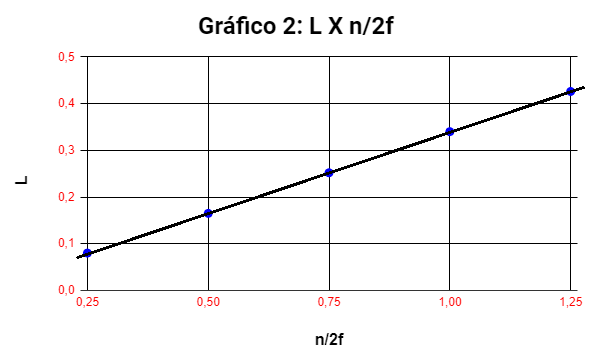
\includegraphics[scale=0.8]{images/Gráfico 2.png}
  \caption{ Gráfico de $L$ em função de $n/2f$.}
\end{figure}

\begin{figure}[H]
  \centering
  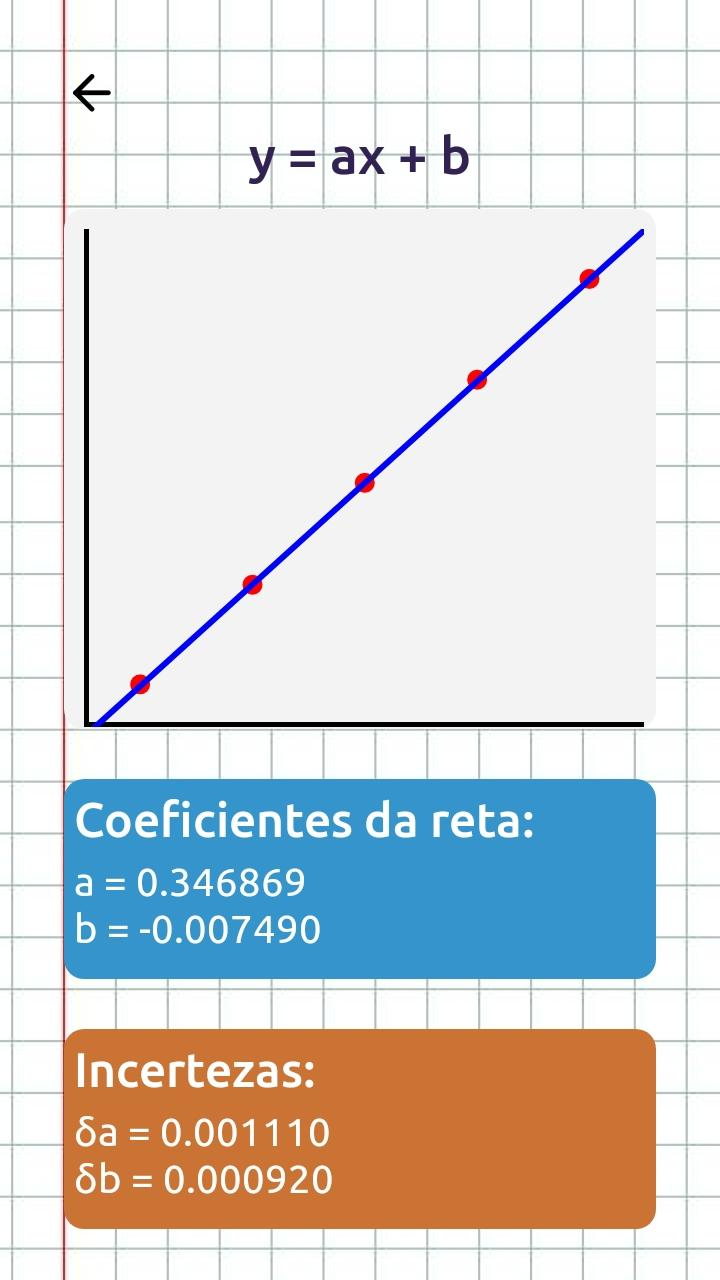
\includegraphics[scale=0.25]{images/Gráfico 2'.jpeg}
  \caption{ Aplicação dos Mínimos Quadrados para obtenção dos coeficientes da reta.}
\end{figure}

Após a análise gráfica da relação entre o comprimento L e o harmônico da onda, aplicando o método dos mínimos quadrados, o coeficiente angular assumiu o valor de a =$(0,347 \pm 0,001)\cdot 10^3$ . Já o coeficiente linear foi igual a: $b =(0,0075 \pm 0,0009)\cdot 10^3$.\\

Dessa forma, como o coeficiente angular corresponde à velocidade na equação de onda estacionária, temos que a velocidade do som no ar, obtido no experimento para uma temperatura local de 25ºC, foi igual a:

\[ \mathbf{\therefore v = (0,347 \pm 0,001) \cdot 10^3 = (347 \pm 1) m/s} \]

Podemos notar que a velocidade obtida por esse método apresentou um valor diferente daquela calculada diretamente da equação. Entretanto, como o valor de referência da velocidade do som no ar corresponde a $v_{ref} = 343$, temos que a velocidade experimental obtida a partir dos mínimos quadrados também não pertence ao intervalo de referência. Assim como no outro método, podemos atribuir essa diferença a erros sistemáticos, porém pode-se notar que o valor atingido também é muito próximo do valor padronizado pela literatura, o que comprova a eficácia experimental.
